\chapter{Overview of the state of the art in graph learning and explainability}
\label{chap:sota}

\section{Machine Learning Tasks on Graphs}

\todo{More general intro on graphs before GNNs}
Graphs are a natural way of abstracting many mathematical problems and a versatile data structure used to represent relationships and interactions in various real-world domains such as chemistry, medicine, particle physics, social networks, medicine, fake-news detection, computer network security, autonomous vehicle guidance and others.\todo{Citations} Consequently, machine learning on graphs has, in recent years, seen an explosion in popularity, breadth and depth of both research and applications.

Let us denote a \name{graph} \( G = \left( V, E \right)) \in \mathcal{G} \) where \( V \) is a set of the graph \name{nodes} and \( E \subseteq V^2 \) is a set of \name{edges} connecting the nodes. The questions of whether the edges should be directed, whether to allow self-loops and/or multiple edges between the same pair of nodes is in general not answered. Most of the discussed methods are agnostic to these choices, which are thus left to the user. Optionally, a vector of \name{node features} \( \mathvec{x}_i \in \mathspace{X} \) may be considered for each node \( v_i \in V \). Additionally, these feature vectors are often considered to form a \name{feature matrix} \( \mathmat{X} \in \mathfield{R}^{\left\lvert V \right\rvert \times \left\lvert \mathspace{X} \right\rvert} \) and this feature matrix is then considered to a part of the graph \( G \). In rare cases, a vector of \name{edge features} \( \mathvec{x}_{ij} \in \mathspace{X} \) is considered as well for all edges \( \left( v_i, v_j \right) \in E \). \todo{More definitions}

While in traditional machine learning, the range of tasks is usually fairly limited, there are four primary ways of applying machine learning algorithms to graph-structured data; node classification, link prediction, learning over the whole graph and community detection. All four of these tasks share some similarities and various machine learning methods on graphs may be applied to multiple tasks or may be adapted from one task to another. However, this is not a universal property with some methods being specific to one task, or even a particular subclass of that task.

\subsection{Node Classification}

Probably the most common task on graphs is that of \name{node classification}, an example of which can be seen in Figure~\ref{fig:node-classification}. In this scenario, a node label \( y_i \in \mathspace{Y} \) is considered for each node \( v_i \in V \). A subset of training nodes \( V_\mathrm{train} \) is typically used to learn a classification function \( f : \mathcal{G} \times V \to \mathspace{Y} \), that is a function taking a graph and one of its nodes and predicting the label of the given node. This function is then used to predict the class of the remaining nodes, using the information about the graph structure encoded in \( G \) and, optionally, the feature matrix \( \mathmat{X} \). \todo{Applications}

\begin{figure}
	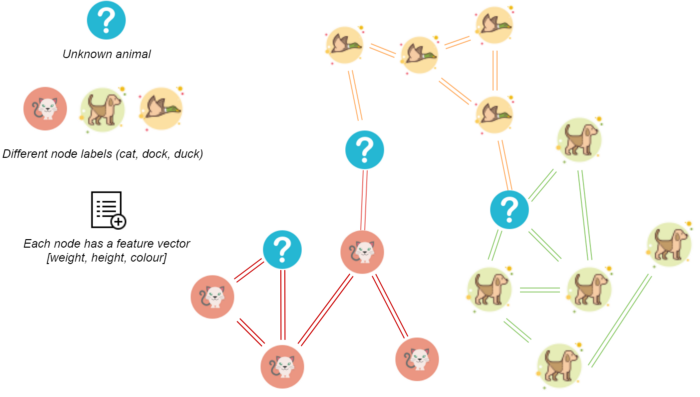
\includegraphics[width=\linewidth]{images/graph-tasks/node-classification.png}
	\caption{A schematic representation of a node classification problem with nodes representing different animals, whose species are the labels of the nodes. Links represent friendships between the different animals. The label is considered to be known for nodes in \( V_\mathrm{train} \) and unknown for other nodes. Original figure from \cite{kubara_machine_2020}.}
	\label{fig:node-classification}
\end{figure}

\subsection{Link Prediction}

The second most common task is that of \name{link prediction}, an example of which is shown in Figure~\ref{fig:link-prediction}. Link prediction focuses on predicting the existence of edges between pairs of nodes in a graph. Given a graph with a set of existing nodes \( E \), the task is to identify potential future or missing edges. This can be framed as a binary classification problem where for each pair of nodes \( (u, v) \in E \), the goal is to predict the probability \( P((u, v) \in E) \). Link prediction is crucial in applications such as recommending friends in social networks, predicting interactions in biological networks, and inferring missing relationships in knowledge graphs.  \todo{References}

\begin{figure}
	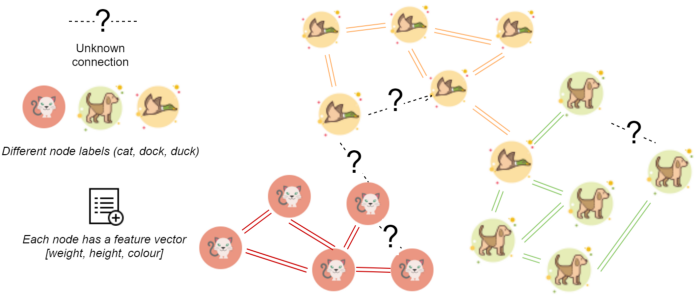
\includegraphics[width=\linewidth]{images/graph-tasks/link-prediction.png}
	\caption{A schematic representation of a link prediction problem with nodes representing different animals, whose species are the labels of the nodes. Links represent friendships between the different animals. Original figure from \cite{kubara_machine_2020}.}
	\label{fig:link-prediction}
\end{figure}

\subsection{Learning over the whole graph}

While node classification and link prediction usually (but not exclusively) concern themselves with tasks within a single graph, it is also possible to consider whole graphs as individual data points. The most common example of this kind of task is \name{graph classification}, where 

Graph classification involves assigning a label to an entire graph rather than individual nodes or edges. Given a set of graphs \( \{G_1, G_2, \ldots, G_N\} \) and corresponding labels \( \{y_1, y_2, \ldots, y_N\} \), the objective is to learn a function \( f: \mathcal{G} \rightarrow \mathcal{Y} \), where \( \mathcal{G} \) denotes the space of all possible graphs and \( \mathcal{Y} \) is the set of labels. This task is common in scenarios where the entire graph structure is indicative of the class, such as in chemical compound classification, where the graph represents the molecular structure, and in document classification, where the graph represents the document's citation or semantic network.

\section{Transductive and inductive learning on graphs}

In the context of machine learning and statistical learning, the terms \name{inductive} and \name{transductive} learning have been used for a long time. In those general fields, the term inductive learning is used for algorithms that use specific training samples to produce general rules, which may then be applied to new samples in the future. In contrast with this stands transductive learning, which foregoes the idea of general rules, instead opting to reason from a set of training samples directly to another set of test samples (see \cite{vapnik_nature_1995}). In the context of graph learning, these two terms are used in a more specific and somewhat different fashion.


\subsection{Inductive Graph Learning}

Inductive graph learning refers to the scenario where the algorithm is trained on a subset of the data and is later evaluated on unseen data. Specifically, the algorithm receives a training set that consists of nodes, edges, labels, and optionally features, and learns a model based on this information. After training, the model is tested on a separate set of data that contains entirely independent nodes, edges, and possibly features, which were not seen during the training phase. When training and test sets are drawn from the same graph, this process is typically achieved by removing the test set from the graph before training. This allows the model to generalize from the training set to new, unseen parts of the graph.

\begin{example}\textbf{Inductive node classification}
	Given a graph \( G = \left( V, E \right) \) with a set of nodes \( V \) and edges \( E \), let \( V_\mathrm{train} \subseteq V \) be the training nodes with known labels, and \( V_\mathrm{test} = V \setminus V_\mathrm{train} \) be the test nodes with unknown labels. The goal in inductive graph learning is to learn the node classification function \( f: \mathcal{G} \rightarrow \mathcal{Y} \) using only \( G \left[ V_\mathrm{train} \right] \), the subgraph of \( G \) induced by \( V_\mathrm{train} \), and \( \mathcal{Y}_\mathrm{train} \), the training node labels. The learned function \( f \) is then evaluated on \( V_\mathrm{test} \).
\end{example}

Inductive methods are more flexible and can handle dynamic and evolving graph structures, making them suitable for applications where the test set is expected to differ from the training set. They are essential for tasks like link prediction in evolving networks or node classification in dynamic environments.

\subsection{Transductive Graph Learning}

Transductive graph learning differs from inductive graph learning in that the algorithm has access to the entire graph, including all nodes, edges, and optionally features, during the training phase. However, the labels for a subset of nodes or edges, referred to as the test set, are withheld. This setting is common in tasks such as node classification and link prediction, where the goal is to infer the missing labels based on the observed graph structure. In transductive learning, the entire graph structure is available during training, but the model only needs to predict the missing labels for the test nodes or edges.

\begin{example}\textbf{Transductive node classification}
	Given a graph \( G = \left( V, E \right) \) where \( V \) is the set of nodes and \( E \) is the set of edges, let \( \mathcal{Y}_\mathrm{train} \) be the labels of the training subset \( V_\mathrm{train} \subseteq V \), and let \( V_\mathrm{test} = V \setminus V_\mathrm{train} \) be the test set of nodes with labels unknown during training. In transductive graph learning, the algorithm aims to learn the node classification function \( f: \mathcal{G} \rightarrow \mathcal{Y} \) that assigns labels to all nodes, utilizing the entire graph structure \( G = \left( V, E \right) \) and the known labels \( \mathcal{Y}_\mathrm{train} \) of the training nodes \( V_\mathrm{train} \). The function \( f \) is then used to predict the labels for the test nodes \( V_\mathrm{test} \).
\end{example}

Transductive methods typically perform well when the test set is not significantly different from the training set, as they can exploit global graph properties and dependencies. However, they usually do not generalize well to new, unseen graphs or nodes.

\section{The graph neural network}\label{sec:gori}

The original \name{Graph Neural Network} (GNN) was first introduced by \cite{gori_new_2005}. While major interest in machine learning on graphs only materialised 10 years later, it is nonetheless this paper that lays the ground work for the entire field. The paper presents a new neural network model called Graph Neural Networks (GNNs), designed to directly process graphs. GNNs extend recurrent neural networks (RNNs) to handle both graph-focused and node-focused applications. The method is based on associating a hidden state vector \( \mathvec{h}_i \in \mathfield{R}^k \) with each node \( v_i \) in the graph, which is updated dynamically according to the node's neighborhood. The update is governed by a parametric transition function \( f_\theta \), which considers the node's label and the states and labels of its neighbors.

Formally, for a graph \( G = (V, E) \), the state \( \mathvec{h}_i \) is defined as the solution to the following system of equations:
\begin{equation}\label{eq:gori-state}
	\mathvec{h}_i = f_\theta \left( y_i, \mathvec{h}_{\mathrm{ne}[v_i]}, y_{\mathrm{ne}[v_i]} \right) , \quad v_i \in V
\end{equation}
where \( y_i \) is the label of node \( v_i \), and \( \mathvec{h}_{\mathrm{ne}[v_i]} \), \( y_{\mathrm{ne}[v_i]} \) represent the states and labels of the neighboring nodes of \( v_i \), respectively. An output vector \( \mathvec{o}_i \in \mathfield{R}^d \) for each node \( v_i \) is defined using a parametric output function \( g_\theta \):
\begin{equation}\label{eq:gori-output}
	\mathvec{o}_i = g_\theta \left( \mathvec{h}_i, y_i \right) , \quad v_i \in V
\end{equation}

Considering for the whole graph a hidden state matrix \( \mathmat{H} \) and a label vector \( \mathvec{y} \), Equations~\ref{eq:gori-state} and~\ref{eq:gori-output} may be rewritten in a stacked form as
\begin{equation}\label{eq:gori-stacked}
	\begin{split}
		\mathmat{H} &= F_\theta \left( \mathmat{H}, \mathvec{y} \right) \\
		\mathmat{O} &= G_\theta \left( \mathmat{H}, \mathvec{y} \right)
	\end{split}
\end{equation}
where \( F_\theta \) and \( G_\theta \) are compositions of \( \left\lvert V \right\rvert \) instances of \( f_\theta \) and \( g_\theta \), respectively. A key observation of the original work is the fact that the Banach fixed point theorem guarantees that if \( F_\theta \) is a contraction mapping, then Equation~\ref{eq:gori-stacked} has a solution and that this solution is unique. Moreover, the theorem states that the following simple iterative system converges exponentially fast to the solution of Equation~\ref{eq:gori-stacked} for any initial state:
\begin{equation}
	\mathmat{H}^{(t+1)} = F_\theta \left( \mathmat{H}^{(t)}, \mathvec{y} \right).
\end{equation}
This allows us to obtain the values of \( \mathvec{h}_i \) and \( \mathvec{o}_i \) by iterating the following system:
\begin{equation}\label{eq:gori-iterative}
	\begin{split}
		\mathvec{h}_i^{(t+1)} &= f_\theta \left( y_i, \mathvec{h}_{\mathrm{ne}[v_i]}^{(t)}, y_{\mathrm{ne}[v_i]} \right) \\
		\mathvec{o}_i^{(t+1)} &= g_\theta \left( \mathvec{h}_i^{(t+1)}, y_i \right)
	\end{split}
\end{equation}

The learning algorithm then consists of two phases:
\begin{itemize}
	\item \textbf{State Computation}: Iteratively update the states \( \mathvec{h}_i^{(t)} \) using Equation~\ref{eq:gori-iterative} until convergence.
	\item \textbf{Parameter Update}: Adapt the parameters \( \theta \) using a gradient descent approach on an error function based on the output and the desired target for a set of training graphs.
\end{itemize}
With the realization of the functions \( f_\theta \) and \( g_\theta \) as feedforward neural networks, the structure of the original Graph Neural Network is complete. Such a GNN model can handle various types of graphs, including directed, undirected, labeled, and cyclic graphs, making it versatile for many practical applications. An example of a simple graph and a corresponding GNN can be seen in Figure~\ref{fig:gori}.

\begin{figure}
	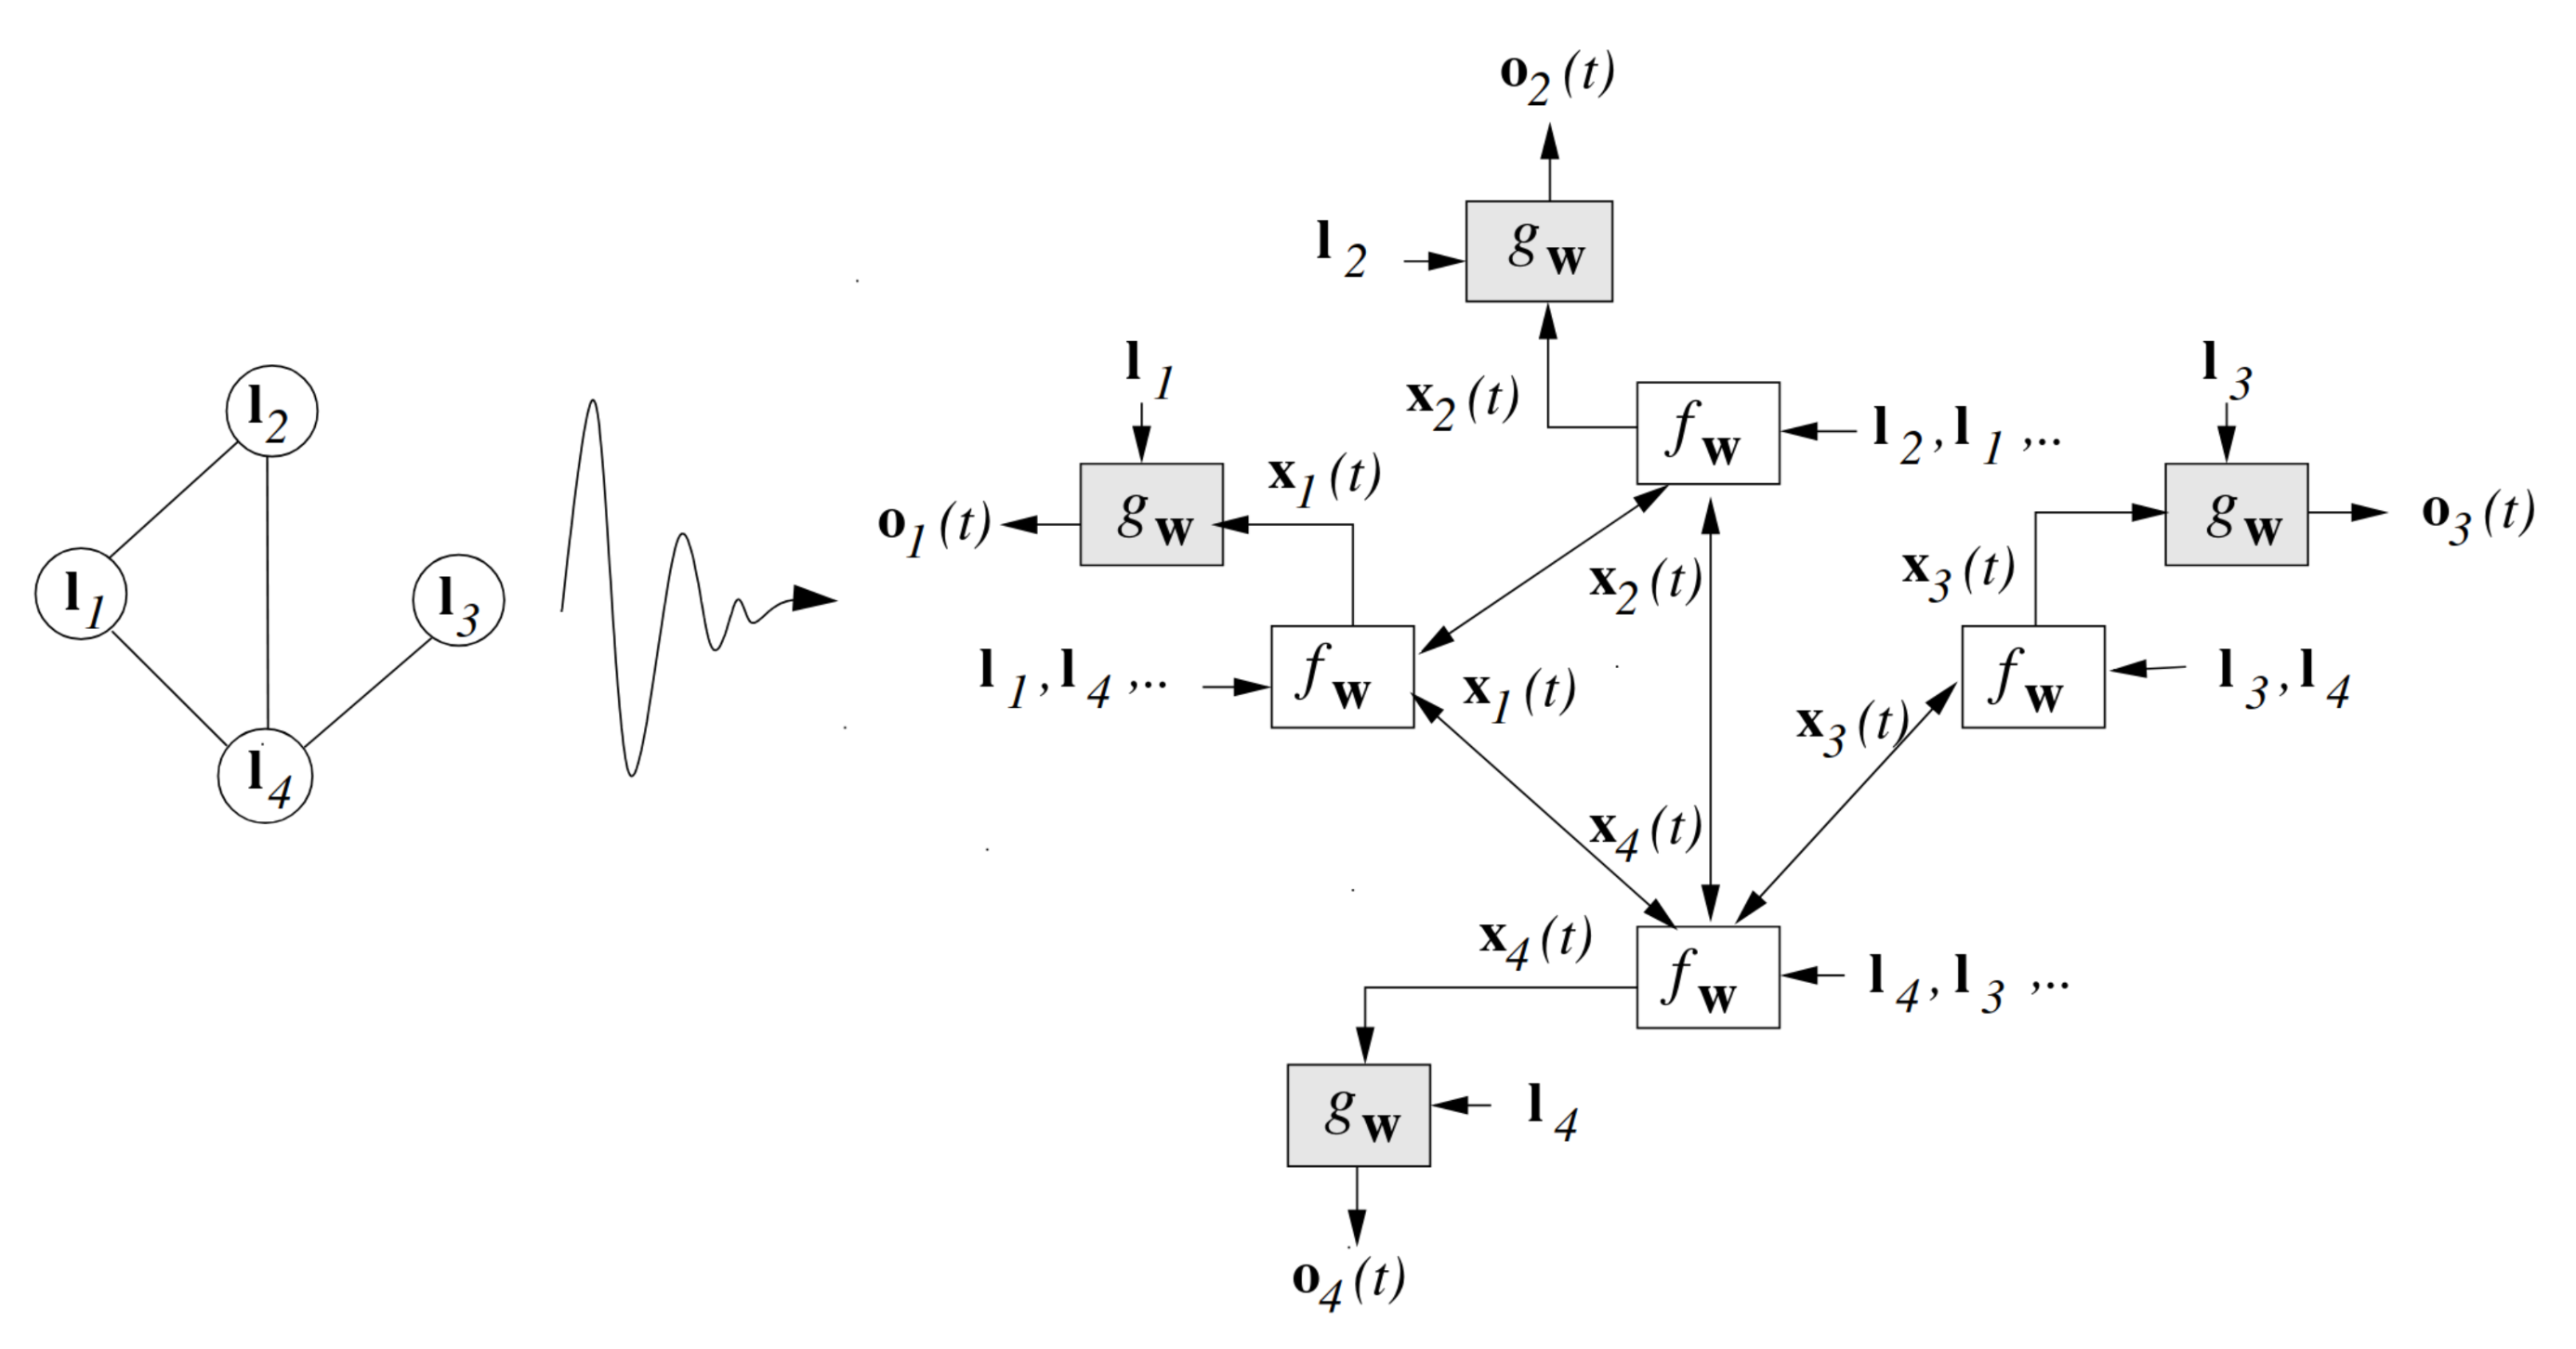
\includegraphics[width=\linewidth]{images/GNN-gori.png}
	\caption{A simple graph with 4 nodes and the corresponding graph neural network. Original figure from \cite{gori_new_2005}. Different notation used, with \( \mathvec{x} \) denoting the hidden state and \( \mathvec{l} \) denoting a node label.}
	\label{fig:gori}
\end{figure}

\section{Random Walk-Based and Convolutional Models for Graph Machine Learning}

Graph machine learning models can be broadly categorized into two main types: random walk-based models and convolutional models.

Random walk-based models utilize random walks to explore the structure of a graph. These models, such as DeepWalk and node2vec, generate sequences of nodes by simulating random paths through the graph. By analyzing these sequences, the models capture the local neighborhood structure and learn low-dimensional embeddings that reflect the relationships between nodes.

Convolutional models, on the other hand, extend the concept of convolution from traditional grid-like data (such as images) to graph data, allowing them to directly leverage the graph structure. Examples of these models include Graph Convolutional Networks (GCNs), Graph Attention Networks (GATs), and GraphSAGE\@. Convolutional models aggregate information from a node’s neighbors to learn representations that capture both local and global graph structure. By stacking multiple convolutional layers, these models can learn increasingly complex patterns and interactions in the graph data, enabling them to make predictions based on the node features and their connections.

Both types of models exploit the graph's topology in different ways to learn meaningful representations of nodes, edges, and the overall graph, allowing for effective predictions and analysis in a variety of applications.

\subsection{Random Walk-Based Models}

Random walk-based models utilize random walks to explore the structure of a graph and understand the relationships between its nodes. A random walk is a process that starts at a given node and moves to a neighboring node at random, continuing this process for a specified number of steps. These walks effectively sample the graph, providing a means to understand the local and, to some extent, global structure of the graph without needing to process the entire graph at once. The following models are, however, all transductive and need to have the whole graph available during training. Due to this, the models can't generalize to samples which were not present during training, as those wouldn't be contained in any of the random walks.

\subsubsection{DeepWalk}

\name{DeepWalk} is one of the pioneering random walk-based methods for learning node embeddings. It treats random walks as equivalent to sentences in natural language processing and applies the Skip-gram model to learn embeddings. See Figure~\ref{fig:deepwalk-motivation} for a motivating example of the similar distributions of word occurrences and vertex occurences in random sequences.

\begin{figure}
	\begin{subfigure}{0.49\linewidth}
		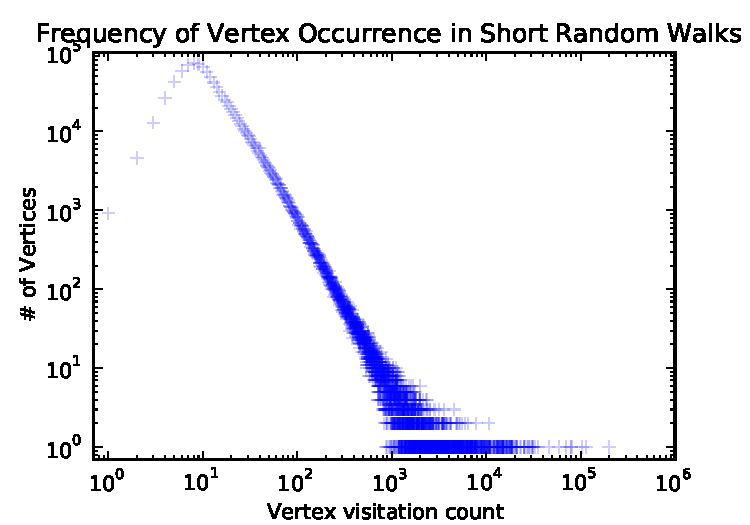
\includegraphics[width=\linewidth]{images/deepwalk-motivation/youtube-powerlaw.pdf}
	\end{subfigure}
	\begin{subfigure}{0.49\linewidth}
		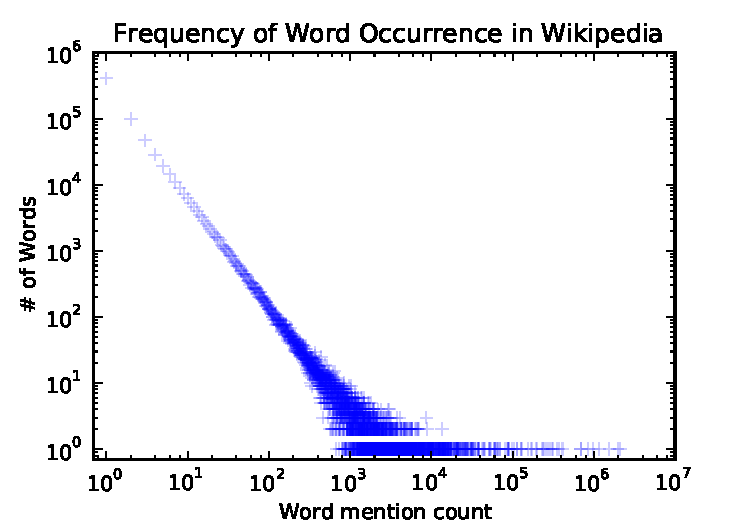
\includegraphics[width=\linewidth]{images/deepwalk-motivation/wiki-powerlaw.pdf}
	\end{subfigure}
	\caption{The distribution of vertices appearing in short random walks follows a power-law, much like the distribution of words in natural language. Original figure from \cite{perozzi_deepwalk_2014}.}
	\label{fig:deepwalk-motivation}
\end{figure}

The DeepWalk algorithm generally consists of two steps -- the generation of random walks from a graph and the extraction of node embeddings from these random walks. The first step is fairly straightforward, the algorithm chooses a random node \( v_i \in V \) as the starting point of the random walk \( \mathcal{W}_{v_i} \) and then constructs the random walk one node at a time by sampling uniformly from the neighbors of the last visited node. This process continues until a desired maximum length \( t \) is reached. In practice, this length is constant across all the random walks generated.

Once a sufficient number of random walks has been generated, these can be used to obtain the node embedding \( \Phi : V \to \mathfield{R}^{\left\lvert V \right\rvert \times d} \). Intuitively, this embedding should maximize the likelihood of observing a given node given all the preceding nodes in the random walk, that is for a random walk \( \mathcal{W} = \left( v_1, v_2, \dots, v_t \right) \), it would maximize
\begin{equation}\label{eq:next-node-probability}
	P \left( v_i \middle| \left( \Phi \left( v_1 \right), \Phi \left( v_2 \right), \dots, \Phi \left( v_{i-1} \right) \right) \right), \quad v_i \in \mathcal{W}
\end{equation}
Computing this objective function, however, quickly becomes unfeasible. Instead, the \name{Skip-gram} algorithm by \cite{mikolov_efficient_2013} is employed. This algorithm, which is visualized in Figure~\ref{fig:skip-gram}, turns the prediction problem on its head by maximizing the probability of preceding nodes in the random walk from the embedding of the current node, instead of Equation~\ref{eq:next-node-probability}. Secondly, instead of only considering the preceding nodes, the algorithm also considers the following nodes. Finally, the order of the nodes in the sequence is disregarded. Together, this gives us the following maximization objective:
\begin{equation}\label{eq:deepwalk-objective}
	P \left( \left\{ v_1, v_2 , \dots, v_{i-1}, v_{i+1}, \dots, v_t \right\} \middle| \Phi \left( v_i \right) \right), \quad v_i \in \mathcal{W}
\end{equation}

\begin{figure}
	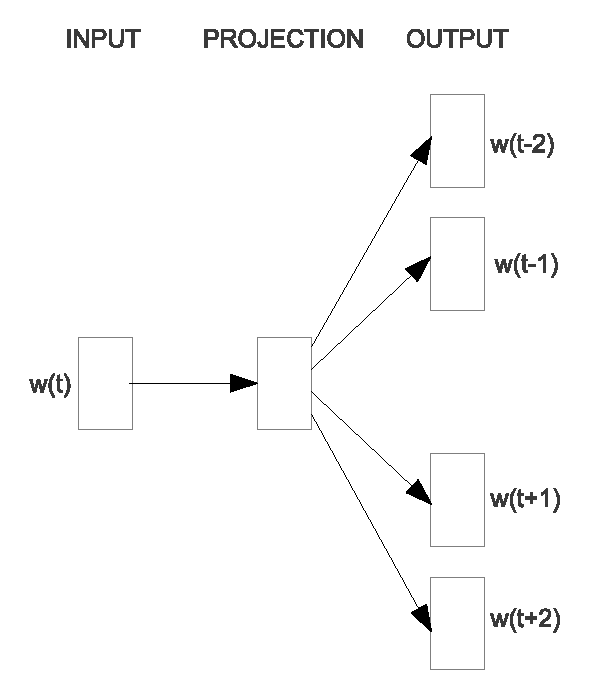
\includegraphics[width=0.6\linewidth]{images/skip-gram.pdf}
	\caption{A schematic representation of the skip-gram algorithm. The embedding (projection) of a word at position \( t \) should maximize the likelihood of surrounding words in the sequence. Original figure from \cite{mikolov_efficient_2013}.}
	\label{fig:skip-gram}
\end{figure}

The algorithm realizes the embedding \( \Phi \) as a matrix of individual node embeddings that is randomly initialized and optimized iteratively over all of the random walks. This optimization is realized as a gradient descent with the objective function being the negative log likelihood of the objective introduced in Equation~\ref{eq:deepwalk-objective}. Further computational optimizations are needed such as a hierarchical softmax algorithm for efficient computation of the node occurence probabilities, however, further details are outside the scope of this work.

\subsubsection{Node2Vec}

\name{Node2vec} is an algorithm designed to learn continuous feature representations of nodes in a graph by optimizing a neighborhood preserving objective. Unlike previous graph embedding techniques such as DeepWalk that often focus solely on structural equivalence, node2vec introduces a flexible notion of a node's neighborhood, allowing it to capture both the homophily and structural equivalence properties of nodes. It achieves this through a biased random walk strategy that balances breadth-first and depth-first graph traversal, thereby capturing diverse patterns in the data. This flexibility enables node2vec to generate representations that are well-suited for various downstream machine learning tasks.

The node2vec algorithm differs from DeepWalk mainly in the way random walks are sampled from the graph, the following extraction of node embeddings is largely the same. Where DeepWalk generated random walks by uniformly sampling among the last node's neighbors in each step, node2vec considers a node's neighborhood \( \mathrm{ne}_S [ v_i ] \) as the primary area of interest, with varying neigbourhood sampling strategies S. To this end, node2vec seeks to maximize the following objective:
\begin{equation}\label{eq:node2vec-objective}
	\sum_{v_i \in V} P \left( \mathrm{ne}_S[v_i] \middle| \Phi \left( v_i \right) \right)
\end{equation}
This objective is simplified further by assuming conditional independence between the likelihoods of observing different neighboring nodes, i.e.
\begin{equation}
	P \left( \mathrm{ne}_S[v_i] \middle| \Phi \left( v_i \right) \right) = \prod_{v_j \in \mathrm{ne}_S[v_i]} P \left( v_j \middle| \Phi \left( v_i \right) \right)
\end{equation}
The choice of the neigbourhood sampling strategy \( S \) is central to node2vec, with the two most extreme options being \name{breadth-first search} (BFS), where \( \mathrm{ne}_S [ v_i ] \) is restricted to immeadiate neighbors of \( v_i \), and \name{depth-first search} (DFS), where nodes are sampled at ever increasing distances from \( v_i \)

Graph representation learning algorithms frequently consider two different kind of node similarities, homophily and structural equivalence. When considering homophily, nodes of the same kind are often connected and relatively close together in the graph, which an embedding obtained with BFS would be able to capture. On the other hand, under structural equivalence, two nodes of the same kind may play the same role withing their respective local neighborhoods, without necessarily being close to one another. An embedding obtained by DFS would be a good representation for such a case. The node2vec random walk generation algorithm is capable of interpolating between BFS and DFS, therefore being suitable for graphs mainly governed by homophily as well as graphs which are better described by structural equivalence.

In order to be able to interpolate between BFS and DFS, the node2vec algorithm considers 2 parameters, \( p \) and \( q \), that control how the random walk is generated. Consider a scenario where the random walk just traversed the edge \( \left( t, v \right) \) and now decides where to continue from the node \( v \). In DeepWalk, the neighbors of \( v_i \) have the same probability \( \frac{1}{\left\lvert \mathrm{ne}[v] \right\rvert} \) of being the next node. With node2vec, this probability is multiplied by a weight \( \alpha_{pq} \left( t, x \right) \) for each candidate node \( x \). This weight is defined as
\begin{equation}\label{node2vec-weight}
	\alpha_{pq} \left( t, x \right) = \begin{cases}
		\frac{1}{p} & \text{for}\ x = t \\
		1 & \text{for}\ x \in \mathrm{ne}[t] \\
		\frac{1}{q} & \text{otherwise.}
	\end{cases}
\end{equation}
This arrangement of weights is schematically visualized in Figure~\ref{fig:node2vec-weights}. By choosing the values of \( p \) and \( q \), this method can easily interpolate between BFS and DFS, for example, by choosing a very high value of \( q \), the random walks are restricted to almost never leave the local neighborhood. DeepWalk can be seen as a special case of node2vec with \( p = q = 1 \).

\begin{figure}
	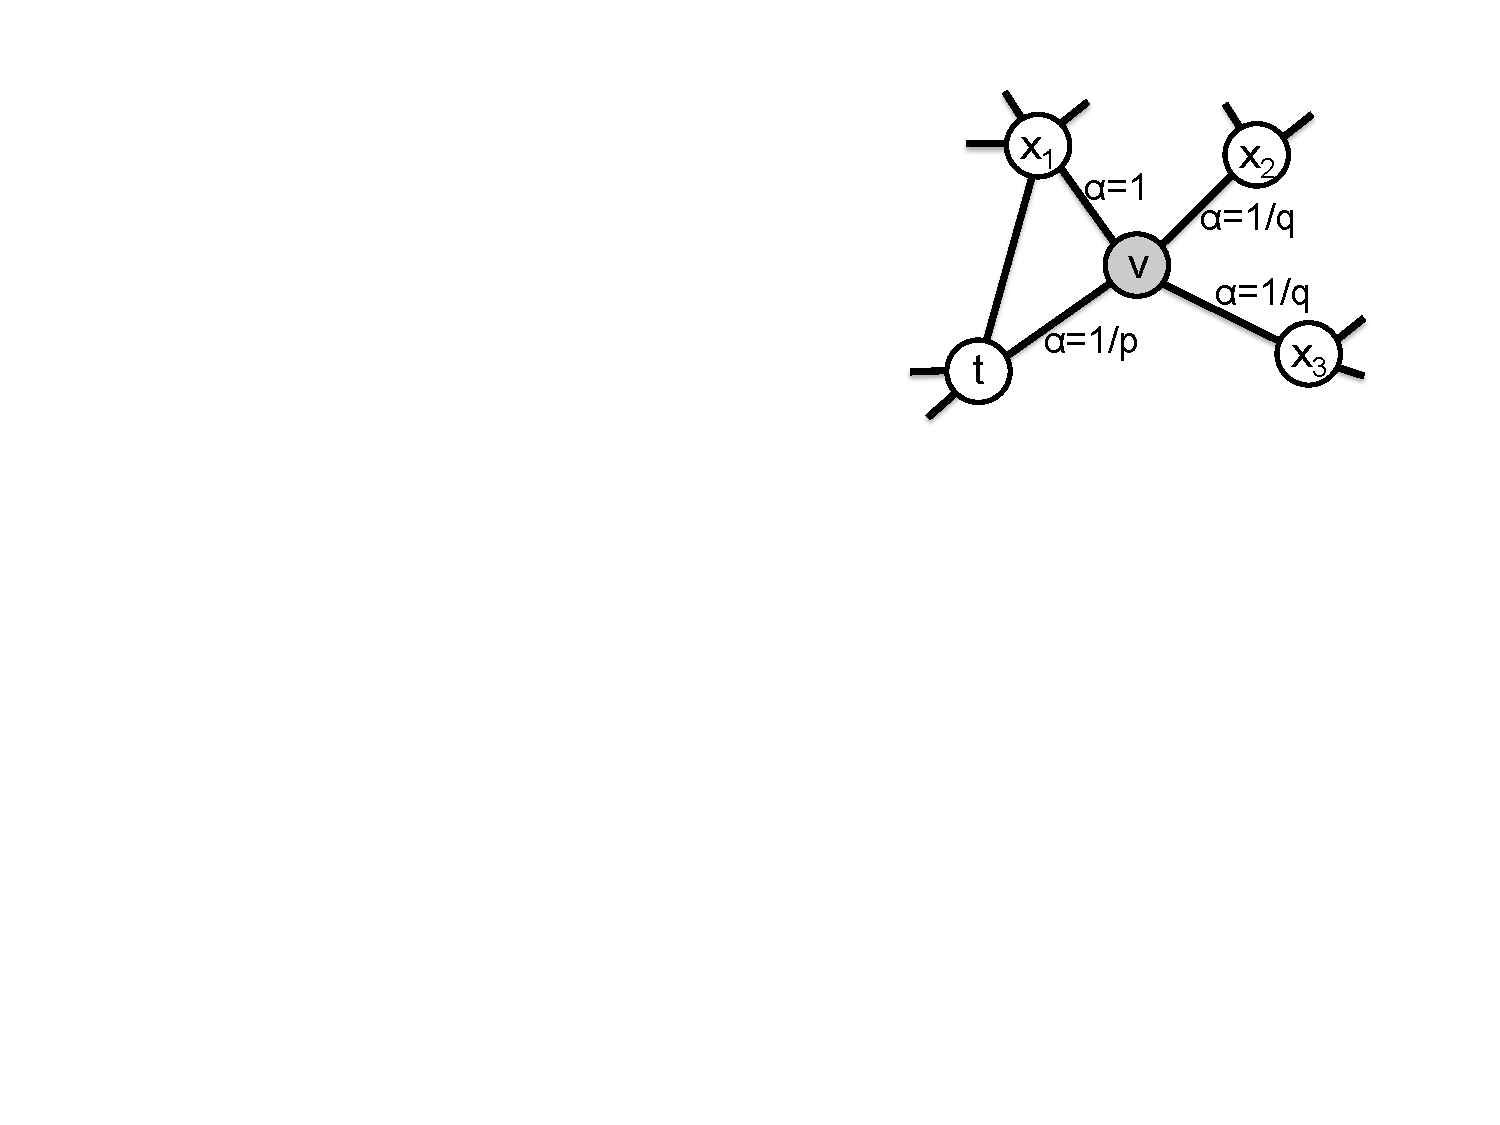
\includegraphics[width=0.6\linewidth]{images/node2vec-weights.pdf}
	\caption{An example of the weights assigned to different nodes in a node2vec random walk. The random walk just traversed from \( t \) to \( v \) and the nodes \( t, x_1, x_2 \) and \( x_3 \) are considered as the next node in the random walk. Original figure from \cite{grover_node2vec_2016}.}
	\label{fig:node2vec-weights}
\end{figure}


\subsection{Convolutional Models}

Convolutional Graph Neural Networks have emerged as a powerful framework for learning on graph-structured data, bridging the gap between traditional graph theory and modern deep learning techniques. At the core of convolutional GNNs lies the Message Passing Neural Network (MPNN) paradigm (see \cite{gilmer_neural_2017}), which provides a flexible and effective mechanism for aggregating information from a node's local neighborhood. This paradigm is inspired by the concept of convolution in image processing, where information from neighboring pixels is combined to learn localized features. Similarly, in the graph domain, the MPNN paradigm allows for the propagation of information across nodes by iteratively exchanging and aggregating messages between neighboring nodes. This process enables the model to capture both local and global structural information within a graph, making it particularly well-suited for tasks such as node classification, graph classification, link prediction, and community detection. By leveraging the inherent relational structure of graphs, convolutional GNNs utilizing the MPNN paradigm have shown remarkable performance across a wide range of applications, from social network analysis to molecular biology, demonstrating their versatility and effectiveness in learning from complex, non-Euclidean data.

The formalisation of the message-passing paradigm is fairly straightforward and in some sense similar to the original GNN as described in Section~\ref{sec:gori}. The message passing process runs for \( T \) time steps and is defined with a message function \( M_t \) and a node update function \( U_t \). A hidden state vector \( \mathvec{h}_i^{(t)} \) is assigned to each node \( v_i \) and updated based on messages \( \mathvec{m}_i^{(t+1)} \) according to
\begin{equation}\label{eq:message-passing}
	\begin{split}
		\mathvec{m}_i^{(t+1)} &= \sum_{v_j \in \mathrm{ne}[v_i]} M_t \left( \mathvec{h}_i^{(t)}, \mathvec{h}_j^{(t)}, \mathvec{x}_{ij} \right) \\
		\mathvec{h}_i^{(t+1)} &= U_t \left( \mathvec{h}_i^{(t)}, \mathvec{m}_i^{(t+1)} \right). \\
	\end{split}
\end{equation}
Both the message function \( M_t \) and the node update function \( U_t \) (as well as an optional readout function converting \( \mathvec{h}_i^{(T)} \) to a final prediction) may be realized in various ways such as feedforward graph neural networks, eigenvectors of the graph Laplacian or non-parametric functions

\subsubsection{Graph Convolutional Networks (GCNs)}

The main idea behind the method presented in the paper \cite{kipf_semi-supervised_2017} is to introduce a scalable and efficient approach for semi-supervised learning on graph-structured data using \name{Graph Convolutional Networks} (GCNs). The authors propose a convolutional architecture that is motivated by a first-order approximation of spectral graph convolutions, which allows their model to efficiently propagate information through the graph by aggregating feature information from a node's neighbors. This layer-wise propagation rule captures both local graph structure and node features, making it particularly well-suited for tasks where labels are only available for a small subset of nodes. The model scales linearly with the number of graph edges, making it computationally efficient and suitable for large-scale graph datasets.

\begin{figure}
	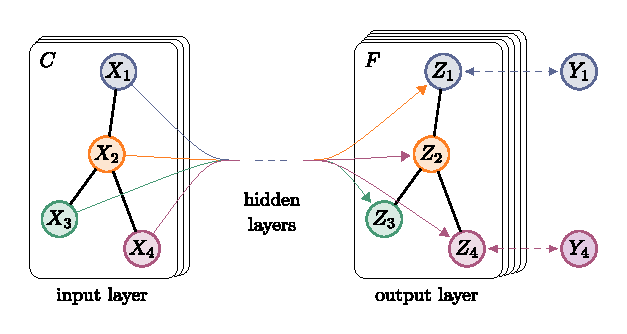
\includegraphics[width=0.8\linewidth]{images/GCN.pdf}
	\caption{Schematic representation of a GCN network learning on a graph with \( C \) input channels and \( F \) output channels. Original figure from \cite{kipf_semi-supervised_2017}.}
	\label{fig:GCN}
\end{figure}

The algorithm for a GCN (schematically represented in Figure~\ref{fig:GCN}) presumes a hidden state matrix \( \mathmat{H}^{(l)} \in \mathfield{R}^{\left\lvert V \right\rvert \times k} \) at layer \( l \) for the whole graph (effectively assigning a \( k \)-dimensional state vector to each node), initialized with the node features of the graph, i.e. \( \mathmat{H}^{(0)} = \mathmat{X} \). The construction of a GCN update step may be viewed as an extension of an ordinary feedforwaard neural network, which would feature a layer update step
\begin{equation}
	\mathmat{H}^{(l+1)} = \sigma \left( \mathmat{H}^{(l)} \mathmat{W}^{(l)} \right)
\end{equation}
where \( \sigma \) is an activation function such as ReLU and \( \mathmat{W}^{(l)} \) are the trainable weights of the \( l \)-th layer. While this structure could theoretically work for a graph dataset, it doesn't actually utilize any of the graph structure. The key insight in GCN is that this may be ameliorated with an addition of the graph adjacency matrix \( \mathmat{A} \) to the update step:
\begin{equation}
	\mathmat{H}^{(l+1)} = \sigma \left( \mathmat{A} \mathmat{H}^{(l)} \mathmat{W}^{(l)} \right).
\end{equation}
This update step, however, does not propagate information contained in a node to the same node in the next layer as the diagonal elements of \( \mathmat{A} \) are zero unless there is a self-loop in that particular node. The authors of GCN propose to improve the update step by replacing the adjacency matrix with the matrix \( \tilde{\mathmat{A}} = \mathmat{A} + \mathmat{I} \), effectively making the model behave as if there were self-loops in each node of the graph. Furthermore, the authors propose to fix one final issue with the method, which is the different magnitude of outputs of each layer depending on the density of edges in the graph. To this end, the pseudo-adjacency matrix \( \tilde{\mathmat{A}} \) needs to be normalized using the diagonal node degree matrix \( \tilde{\mathmat{D}} \) defined as \( \tilde{\mathmat{D}}_{ii} = \sum_j \tilde{\mathmat{A}}_{ij} \). The normalization is carried out in a symmetric fashion, yielding the final update rule
\begin{equation}\label{eq:GCN}
	\mathmat{H}^{(l+1)} = \sigma \left( \tilde{\mathmat{D}}^{-\frac{1}{2}} \tilde{\mathmat{A}} \tilde{\mathmat{D}}^{-\frac{1}{2}} \mathmat{H}^{(l)} \mathmat{W}^{(l)} \right).
\end{equation}
The choices behind the specific modifications of the simple update rule are further theoretically motivated in \cite{kipf_semi-supervised_2017}. The update rule corresponds to a message passing rule defined by
\begin{equation}
	\begin{split}
		M_t \left( \mathvec{h}_i^{(t)}, \mathvec{h}_j^{(t)} \right) &= \left( \mathdeg \left( v_i \right) \mathdeg \left( v_j \right) \right)^{-\frac{1}{2}} \tilde{\mathmat{A}}_{ij} \mathvec{h}_j^{(t)} \\
		U_t \left( \mathvec{h}_i^{(t)}, \mathvec{m}_i^{(t+1)} \right) &= \sigma \left( \mathmat{W}^{(t)} \mathvec{m}_i^{(t+1)} \right). \\
	\end{split}
\end{equation}
Seeing as each layer of GCN aggregates to each node messages from its 1-hop neighborhood, the amount to which the algorithm is concerned with the local neigbourhood of each node versus the global structure of the graph can be controlled by the number of GCN layers. To achieve sufficient expressive power, the GCN layers are frequently used in conjunction with subsequent feedforward layers that further process the information aggregated by the convolutional part in each node independently.

\subsubsection{GraphSAGE}

Low-dimensional embeddings of nodes in graphs are critical for numerous predictive tasks, such as content recommendation and protein function identification. All of the previous methods for generating these embeddings are transductive, relying on a fixed graph structure known at training time. However, real-world applications often require inductive capabilities, meaning embeddings must be generated for unseen nodes or new graphs. To address this, the GraphSAGE (SAmple and AggreGatE) framework introduces an inductive approach that utilizes node feature information to generate embeddings for nodes in unseen data, overcoming the limitations of previous methods.

\begin{figure}
	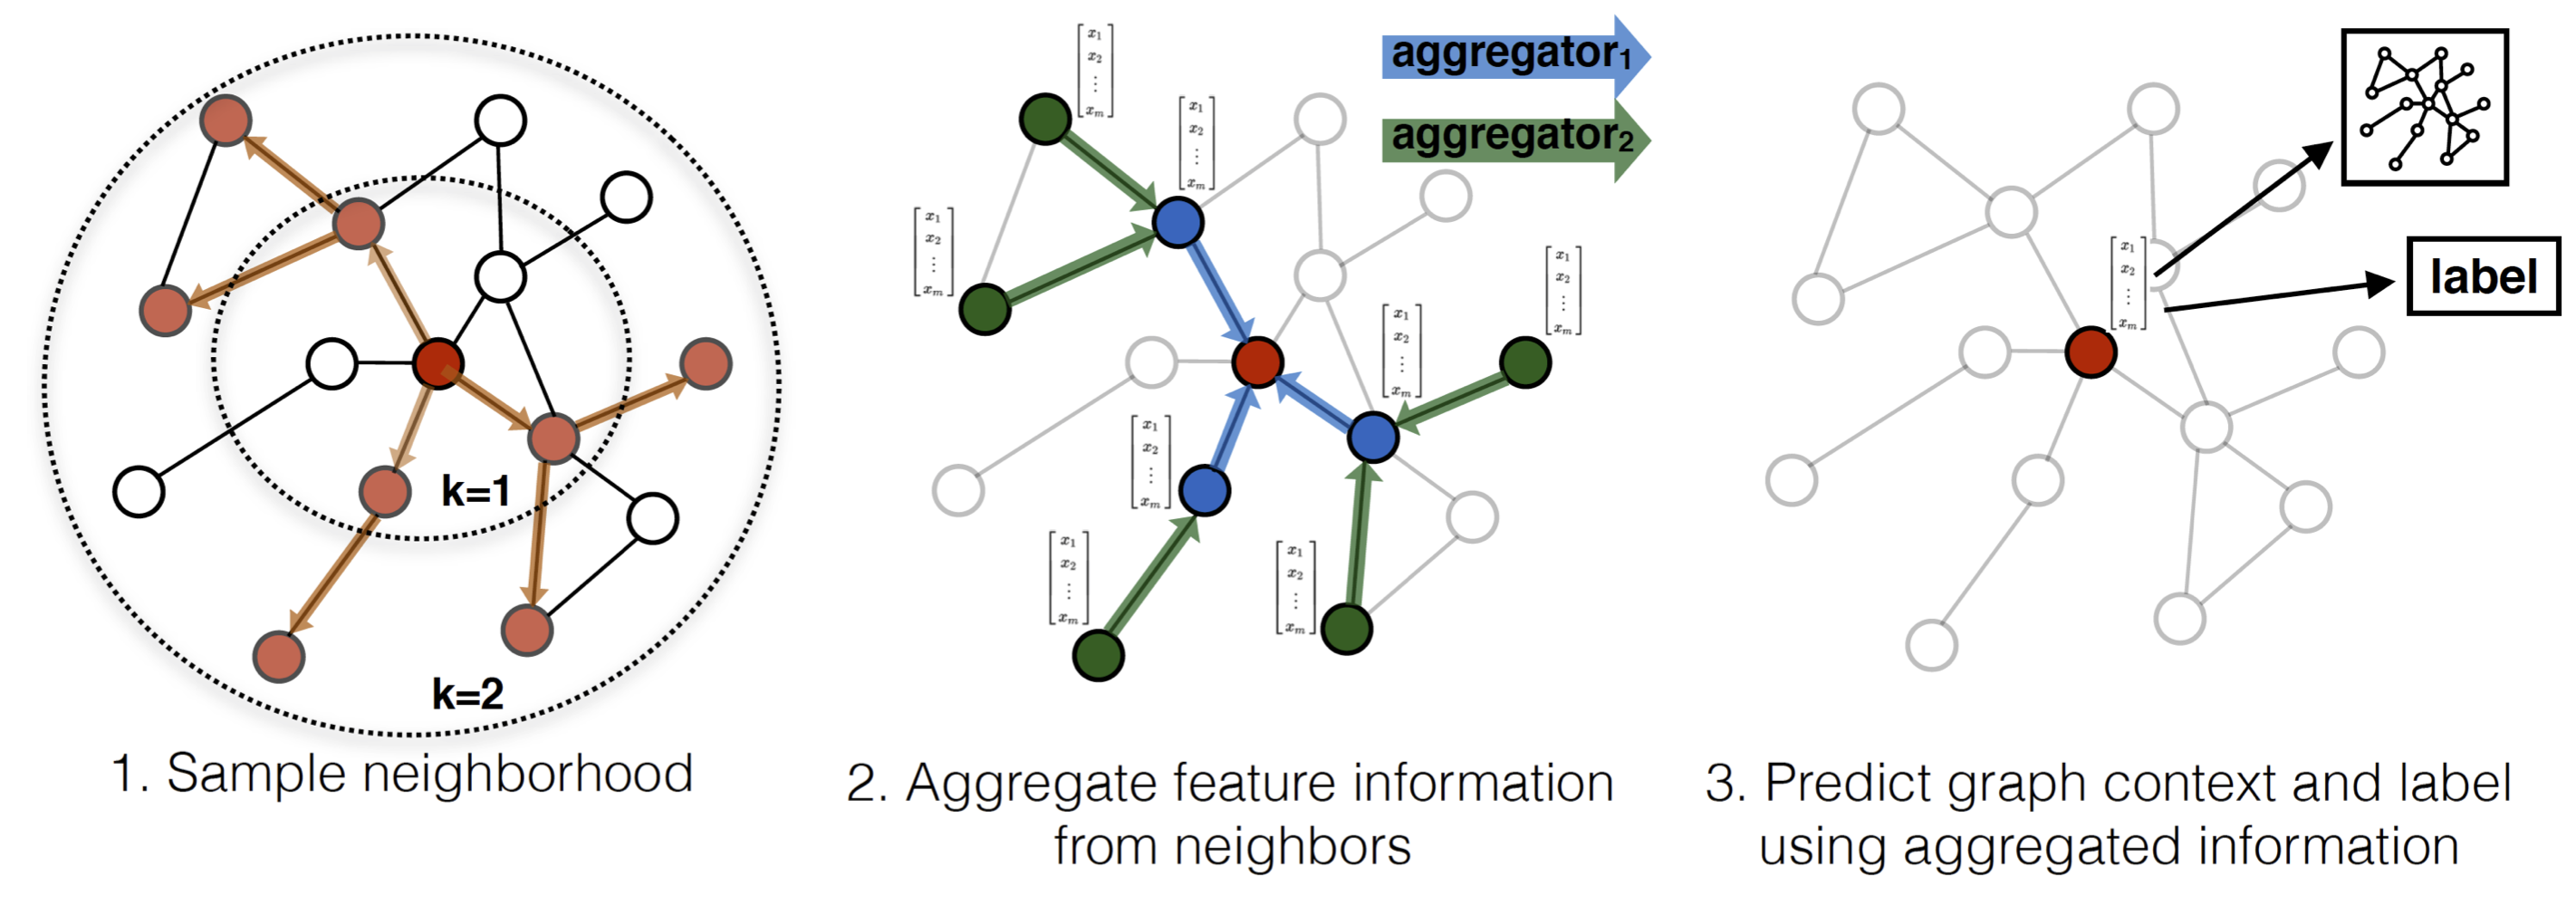
\includegraphics[width=\linewidth]{images/GraphSAGE.png}
	\caption{Schematic representation of a GraphSAGE sampling, aggregation and inference. Original figure from \cite{hamilton_inductive_2017}.}
	\label{fig:GraphSAGE}
\end{figure}

GraphSAGE generates embeddings by learning aggregation functions that sample and aggregate features from a node’s local neighborhood. Instead of learning embeddings for each node, GraphSAGE learns a function that can generate embeddings on-the-fly for any node, whether it has been seen during training or not. This function is trained using node feature information and structural properties of the graph. The process is schematically visualized in Figure~\ref{fig:GraphSAGE} and works in two steps -- neigborhood sampling and feature aggregation.

In contrast to previous methods such as GCN, the GraphSAGE algorithm doesn't use the full neigborhood set, instead opting to uniformly size a fixed-size set of neighbors for each node. This gives for each node \( v_i \) a neigborhood sample \( \mathcal{N} \left( v_i \right) \). This sampling incidentally also constraints the computational complexity of the algorithm, which is \( \mathcal{O} \left( \left\lvert V \right\rvert \right) \) for GCN and \( \mathcal{O} \left( K \right) \) for GraphSAGE, where \( K \) is a constant depending only on method hyperparameters (one of which is the size of the neighborhood sample).

To aggregate the features of the graph, GraphSAGE, like many other methods, operates with a vector \( \mathvec{h}_i^{(l)} \) representing the hidden state assigned to node \( v_i \) in layer \( l \). On top of this, another vector \( \mathvec{h}_{\mathcal{N} \left( v_i \right)}^{(l)} \) is introduced, representing the hidden state assigned to the neigborhood of \( v_i \). The iterative process is then described by the following system
\begin{equation}
	\begin{split}
		\mathvec{h}_{\mathcal{N} \left( v_i \right)}^{(l)} &= \mathrm{AGGREGATE}_l \left( \left\{ \mathvec{h}_j^{(l-1)} \middle| v_j \in \mathcal{N} \left( v_i \right) \right\} \right) \\
		\mathvec{h}_i^{(l)} &= \sigma \left( \mathmat{W}^{(l)} \cdot \mathrm{CONCAT} \left( \mathvec{h}_i^{(l-1)}, \mathvec{h}_{\mathcal{N} \left( v_i \right)}^{(l)} \right) \right) \\
	\end{split}
\end{equation}
where \( \mathrm{AGGREGATE}_l \) is a configurable aggregation function. In theory, this aggregator can be different for each layer, in practice, this is rarely used and the aggreagators are kept the same for all layers. There are several proposed realizations of the aggreagator:
\begin{itemize}
	\item \textbf{Mean aggregation}: An aggregator that uses simple element-wise averaging all the neighboring node hidden states. This yields a method that is equivalent to GCN, however, due to the neigborhood sampling, the GraphSAGE variant is an inductive method instead of a transductive one.
	\item \textbf{LSTM aggregation}: A LSTM module may also be used to aggregate the hidden states, which gives the model greater expressive power compared to the mean aggregation. Of note is the fact that the nodes need to be randomly permuted as the LSTM model is not inherently permutation invariant.
	\item \textbf{Pooling aggregation}: As an alternative to the LSTM model, a single layer feedforward model may be also used together with element-wise max pooling (or any other pooling operator). This approach is reminiscent of the aggregation often used in multi-instance learning (see \cite{dietterich_solving_1997}).
\end{itemize}

In summary, GraphSAGE represents a significant advancement in the field of graph-based machine learning, providing a robust framework for inductive node embeddings that generalize to new graphs and unseen nodes. By leveraging node features and a flexible aggregation mechanism, GraphSAGE can efficiently produce embeddings that are useful for various downstream tasks, thus making it a valuable tool for evolving, real-world applications.

\todo[inline,caption={}]{If there is time: WL test and expressivity in GNNs
	\begin{itemize}
		\item The WL test
		\item The WL test and graph convolution
		\item GIN?
		\item Oversmoothing in graphs
		\item Oversquashing in graphs
		\item The 4 Gs?
	\end{itemize}
}

\section{Explainability in Graph Learning}

In recent years, explainability has emerged as a crucial area of research, particularly in the context of machine learning models applied to graph-structured data. As these models become more complex and are deployed in critical applications -- ranging from social network analysis to biological network exploration and financial fraud detection -- the ability to interpret and understand their predictions is increasingly important. Explainability in graph models not only enhances trust and transparency but also facilitates debugging and improves model performance by identifying biases or errors in data. This section delves into various methodologies for explaining graph-based models, highlighting key techniques and tools that have been developed to interpret their outputs effectively. We will explore approaches that elucidate the decision-making processes of these models, ensuring their predictions are comprehensible and reliable to both experts and non-experts alike.

Over the recent years, a large number of graph explanation algorithms has been proposed. \cite{yuan_explainability_2022} propose a taxononomy of the various methods, which is shown in Figure~\ref{fig:graph-explainability-taxonomy}. The taxonomy arranges the methods into 2 main categories -- instance-level explanations and model-level explanations. Instance level explanations aim to explain the prediction of a particular instance (node, graph, etc.) on which the underlying graph algorithm was applied. These methods are further classified based on the method they use to obtain such explanations. In contrast, graph-level explanations aim to explain the inner workings of a graph model without respect to any individual example. In the rest of this section, several explanation methods are introduced.

\begin{figure}
	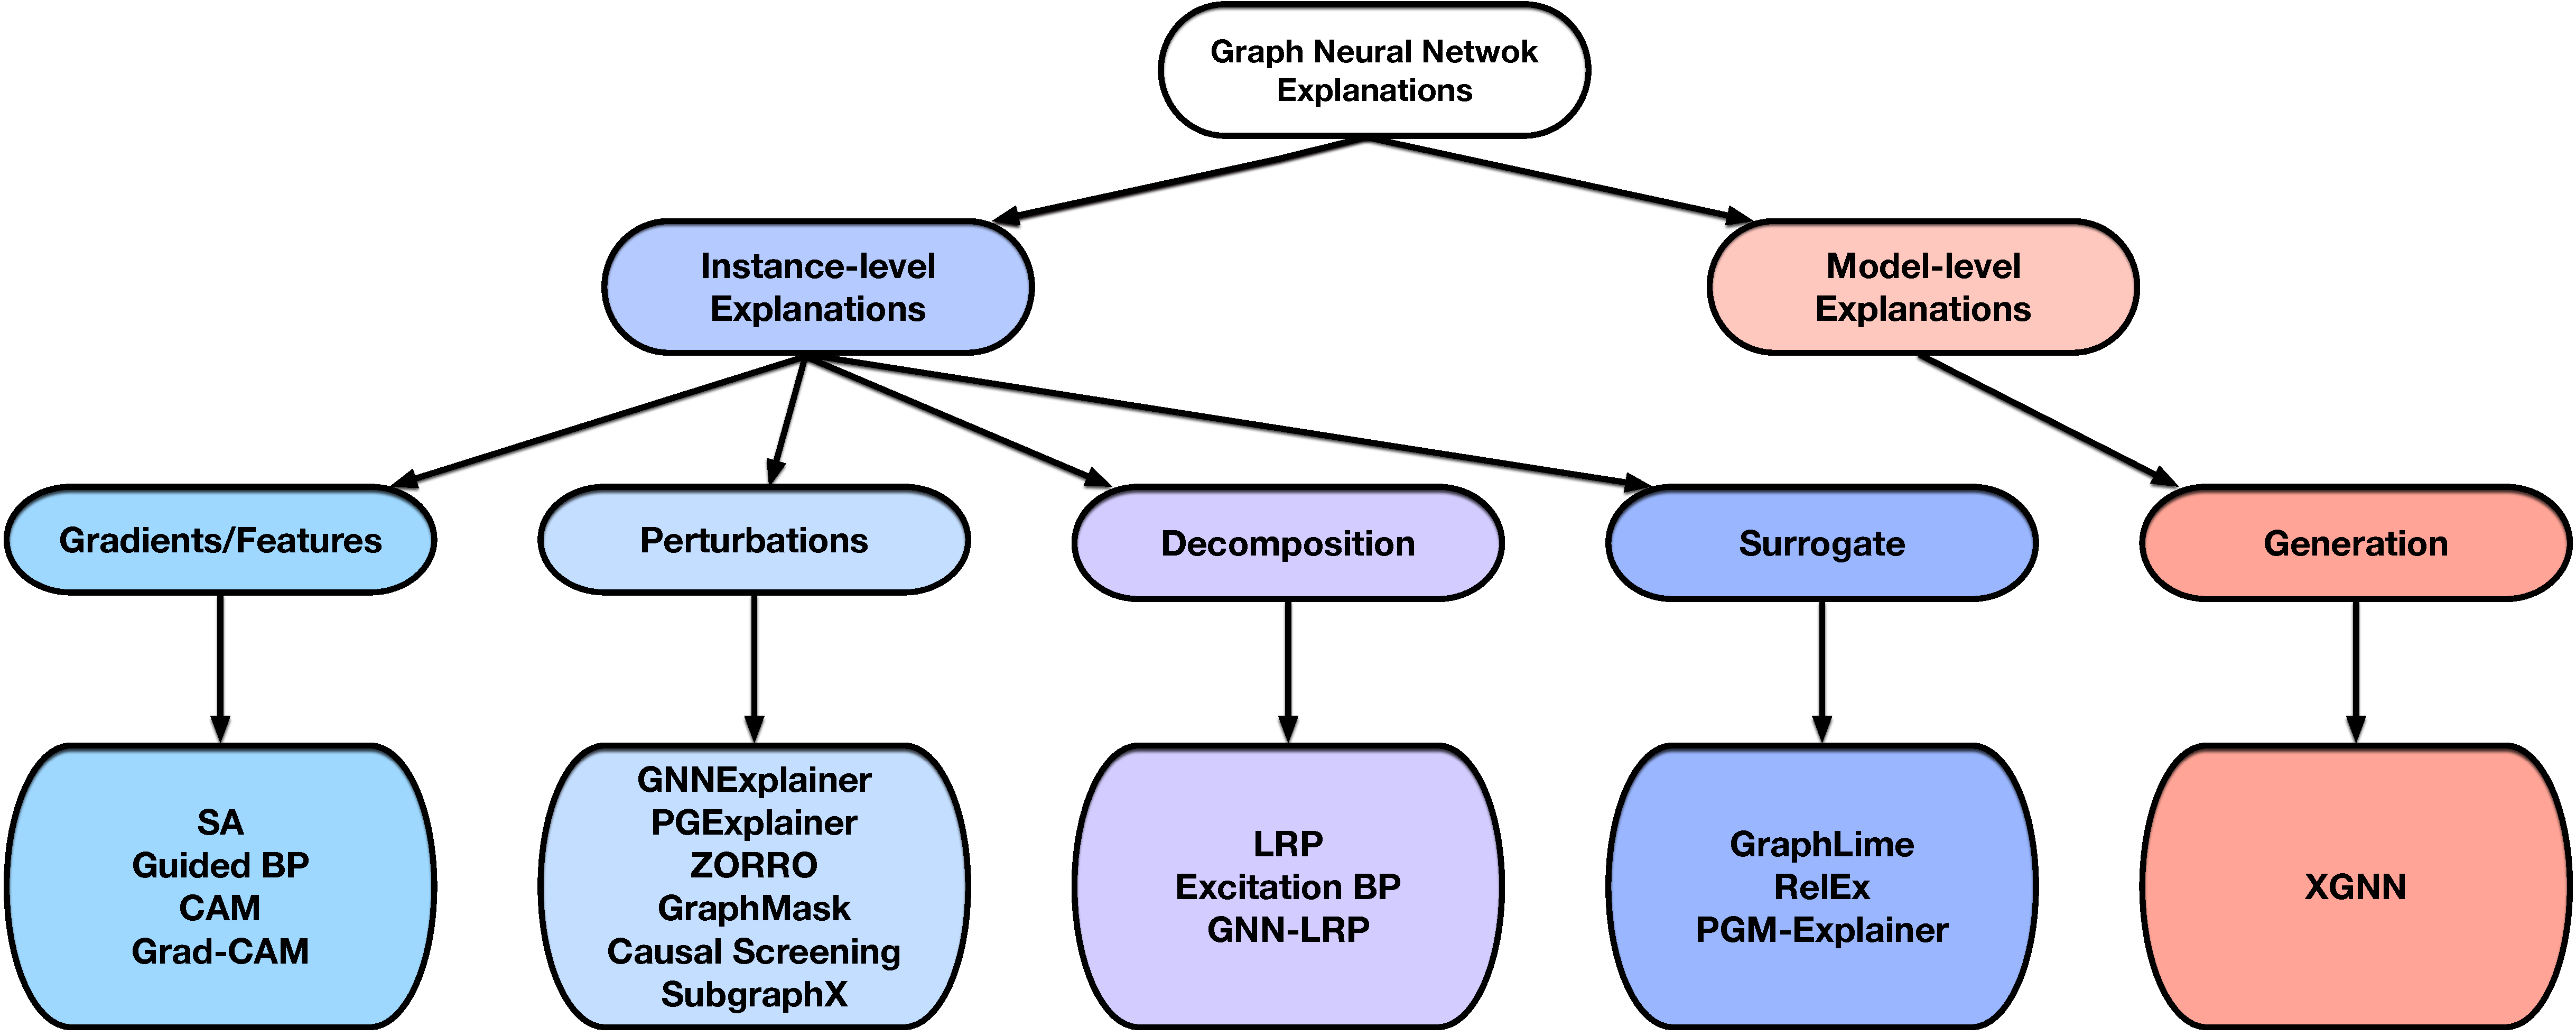
\includegraphics[width=\linewidth]{images/graph-explainability-taxonomy.pdf}
	\caption{An overview of the taxonomy of graph explainability methods. Original figure from \cite{yuan_explainability_2022}.}
	\label{fig:graph-explainability-taxonomy}
\end{figure}

\todo[inline]{Gradient-based instance-level methods -- Grad-CAM}

\subsection{Surrogate methods}

Complex models such as GNNs are difficult to explain due to the complicated and nonlinear relationships between the input space and output predictions. A common approach for instance-level explanations in image models is the surrogate method. This involves using a simple, interpretable model to approximate the predictions of a more complex deep model in the local area around a specific input. The explanations generated by the surrogate model are then used to explain the original prediction. However, applying surrogate methods to graph data is challenging because graphs are discrete and contain topological information, making it unclear how to define neighboring regions of the input graph and which interpretable models are suitable.

\subsubsection{GraphLIME}

\name{GraphLIME} is a model-agnostic, local interpretability framework specifically designed for GNNs, introduced by \cite{huang_graphlime_2023}. It extends the LIME approach by using the Hilbert-Schmidt Independence Criterion (HSIC) Lasso, a non-linear feature selection method, to better capture the dependencies in graph-structured data. Unlike traditional methods that use linear approximations, GraphLIME employs a non-linear explanation model, making it more effective for explaining GNN predictions.

GraphLIME is a generalization of the LIME explanation algorithm (see \cite{ribeiro_why_2016}). The main advance over LIME is the selection of a local neighborhood, which is needed by LIME in order to select a surrogate model that matches the predictions of the GNN on a local neighborhood. To achieve this when explaining the prediction of the node \( v_i \), GraphLIME looks at the \( N \)-hop neighborhood \( \mathcal{S}_N \left( v_i \right) \), that is the set of nodes from which exists a path to \( v_i \) consisting of no more than \( N \) edges. When such a neighborhood is found consisting of nodes \( \mathcal{S}_N \left( v_i \right) = \left\{ v_{j_1}, v_{j_2}, \dots, v_{j_N} \right\} \), the set of their corresponding feature vectors and predicted labels from the underlying GNN \( \left\{ \left( \mathvec{x}_{j_k}, \hat{y}_{j_k} \right) \right\}_{k=1}^{N} \) is used as the local dataset to train the surrogate model on. This model is the Hilbert-Schmidt Independence Criterion (HSIC) Lasso (see \cite{yamada_high-dimensional_2014}), a kernel-based feature-selection algorithm. Therefore, the output of the GraphLIME algorithm is a list of features important to the instance being explained, without any explanation of how the local structure of the graph contributes to the prediction.

\begin{itemize}
	\item Overview of graph explainability
		\begin{itemize}
			\item Perturbation-based methods
				\begin{itemize}
					\item GNNExplainer
					\item PGExplainer
					\item SubgraphX
				\end{itemize}
		\end{itemize}
	\item Model-level explainability
		\begin{itemize}
			\item XGNN
			\item GraphChef?
		\end{itemize}
\end{itemize}
